\chapter{Platform-specific reference implementations}

\section{Engineering principles}

Three deployment profiles share one task contract and verification pipeline: Codex implementation, Claude Code implementation, and hybrid implementation followed by read-only review from the second platform. Each profile uses native CLI interfaces and avoids reinventing the agent reasoning loop. The hybrid profile is an external orchestration pattern; it does not imply a native cross-vendor protocol.\src{O1,O4,A1,A6,O8,A7}

\section{Implementation approach}

Use the examples directory as a disposable Git project. Run the local unit tests first. Install and authenticate each CLI outside the task workspace, pin versions, and validate effective policy. Copy the reviewed skills and platform configuration into the target repo. Run the orchestrator with a task file and provider selection; the mock provider exercises the workflow without credentials. Review the diff and verification report before any commit. For hybrid, run the reviewer in a separate read-only checkout and treat its text as advisory.

\section{Verification and limitations}

The prototype deliberately does not merge, push, deploy or accept an agent-supplied approval. Its path check is a postcondition, not containment. Production adoption requires OS isolation, trusted verifier execution and authenticated external approval.

Figure~\ref{fig:d24} illustrates the conceptual flow from Task contract to Trusted verifier. The edges describe the proposed integration or control relationship, not undocumented internal calls.

\begin{figure}[htbp]\centering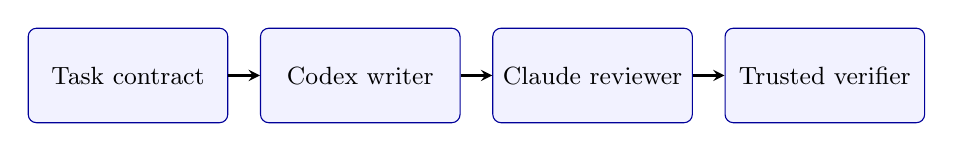
\begin{tikzpicture}[nodebox/.style={draw=blue!60!black,fill=blue!5,rounded corners=3pt,minimum height=12mm,text width=23mm,align=center,font=\small},>=stealth]
\node[nodebox] (n0) at (0.00,0.00) {Task contract};
\node[nodebox] (n1) at (2.95,0.00) {Codex writer};
\node[nodebox] (n2) at (5.90,0.00) {Claude reviewer};
\node[nodebox] (n3) at (8.85,0.00) {Trusted verifier};
\draw[->,thick] (n0.east) -- (n1.west);
\draw[->,thick] (n1.east) -- (n2.west);
\draw[->,thick] (n2.east) -- (n3.west);
\end{tikzpicture}
\caption{Hybrid Codex and Claude Code (conceptual view).}\label{fig:d24}\end{figure}

\section{Chapter conclusion}

Apply the stated verification criteria before expanding the scope of this workflow. Record deviations, evidence and unresolved risks in the task record.
